\section{Ergebnisse} % (fold)
    \label{sec:ergebnisse}
    \subsection{UniRef90 Sampling} % (fold)
        \label{sub:uniref90_results}
        \begin{figure}[H]
            \centering
            \begin{subfigure}{.45\textwidth}
                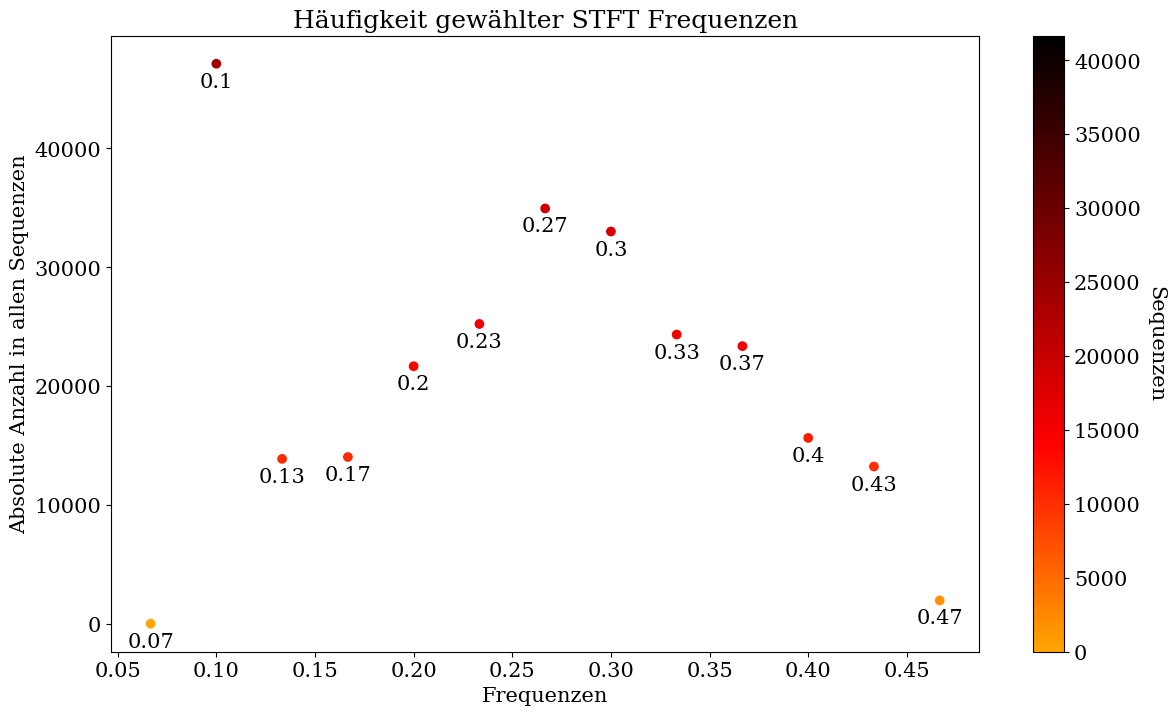
\includegraphics[width=\textwidth]{frequencies_5.png}
                \caption{$\alpha=5\%$}
                \label{fig:frequencies_5}
            \end{subfigure}
            \begin{subfigure}{.45\textwidth}
                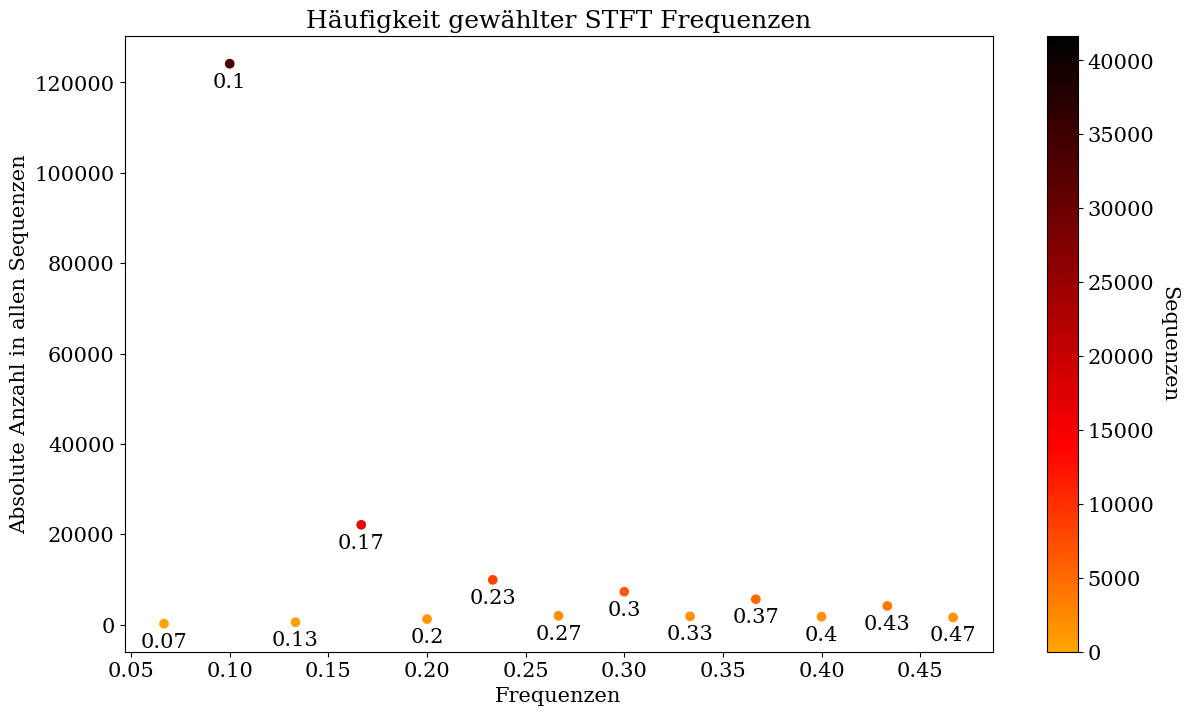
\includegraphics[width=\textwidth]{frequencies_0.1.png}
                \caption{$\alpha=0.1\%$}
                \label{fig:frequencies_0.1}
            \end{subfigure}\\
            \begin{subfigure}{.45\textwidth}
                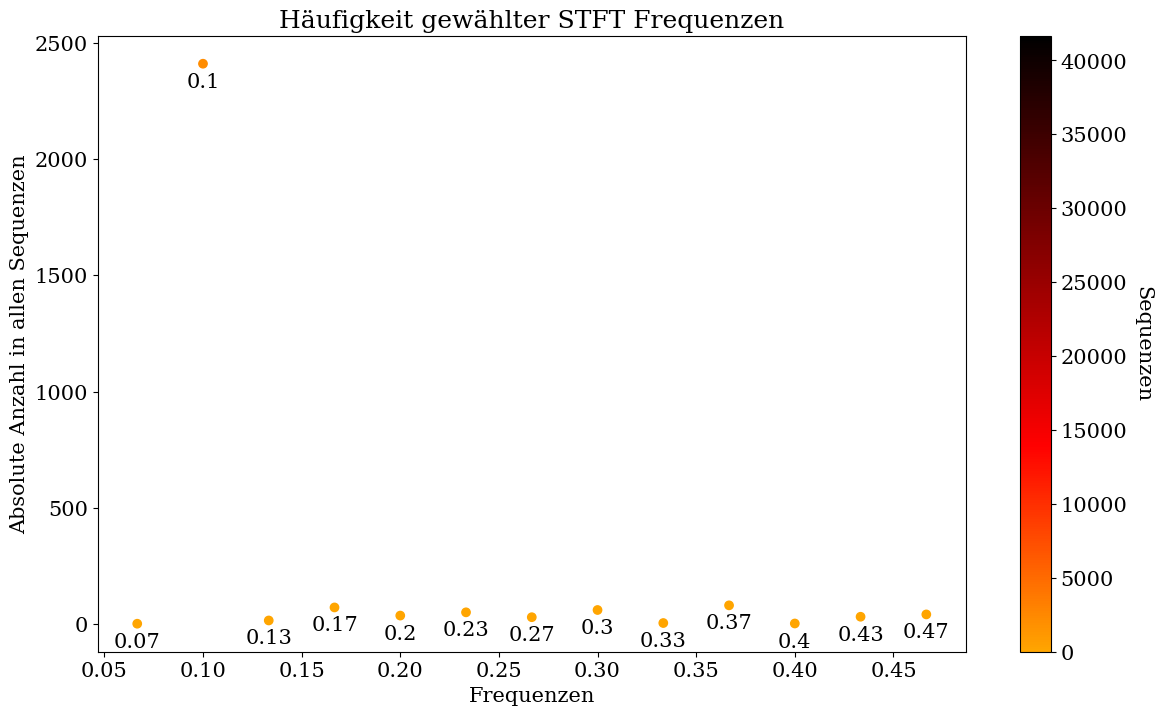
\includegraphics[width=\textwidth]{frequencies_0.01.png}
                \caption{$\alpha=0.01\%$}
                \label{fig:frequencies_0.01}
            \end{subfigure}
            \begin{subfigure}{.45\textwidth}
                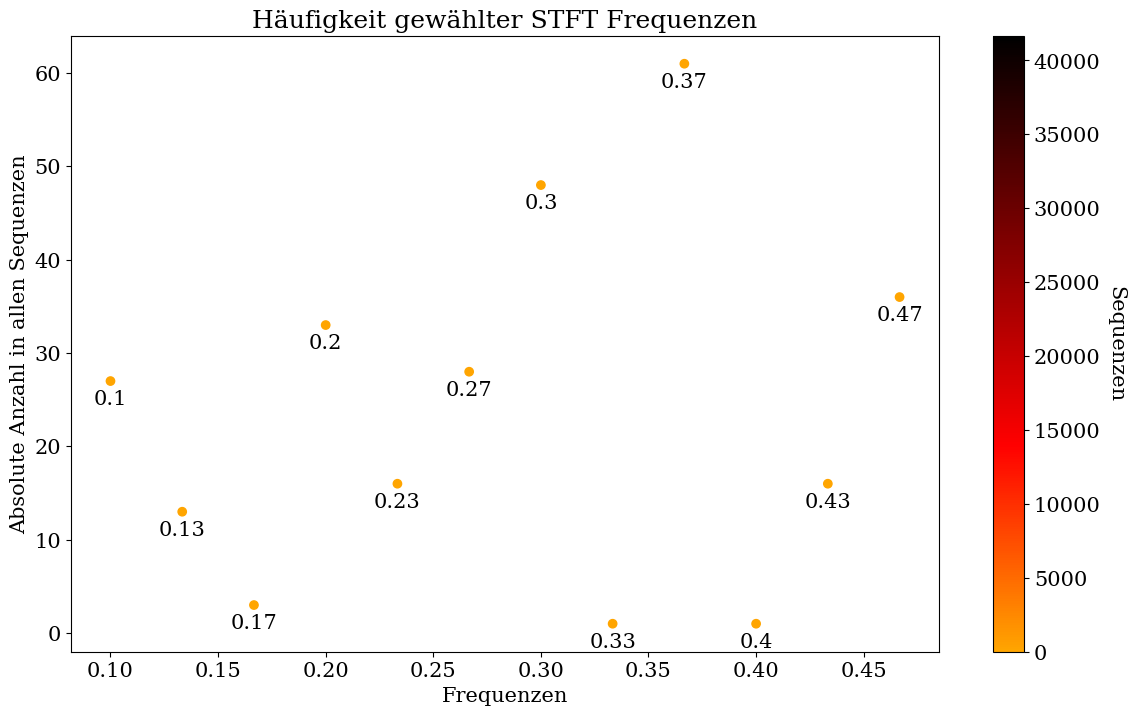
\includegraphics[width=\textwidth]{frequencies_0.001.png}
                \caption{$\alpha=0.001\%$}
                \label{fig:frequencies_0.001}
            \end{subfigure}\\
            \begin{subfigure}{.45\textwidth}
                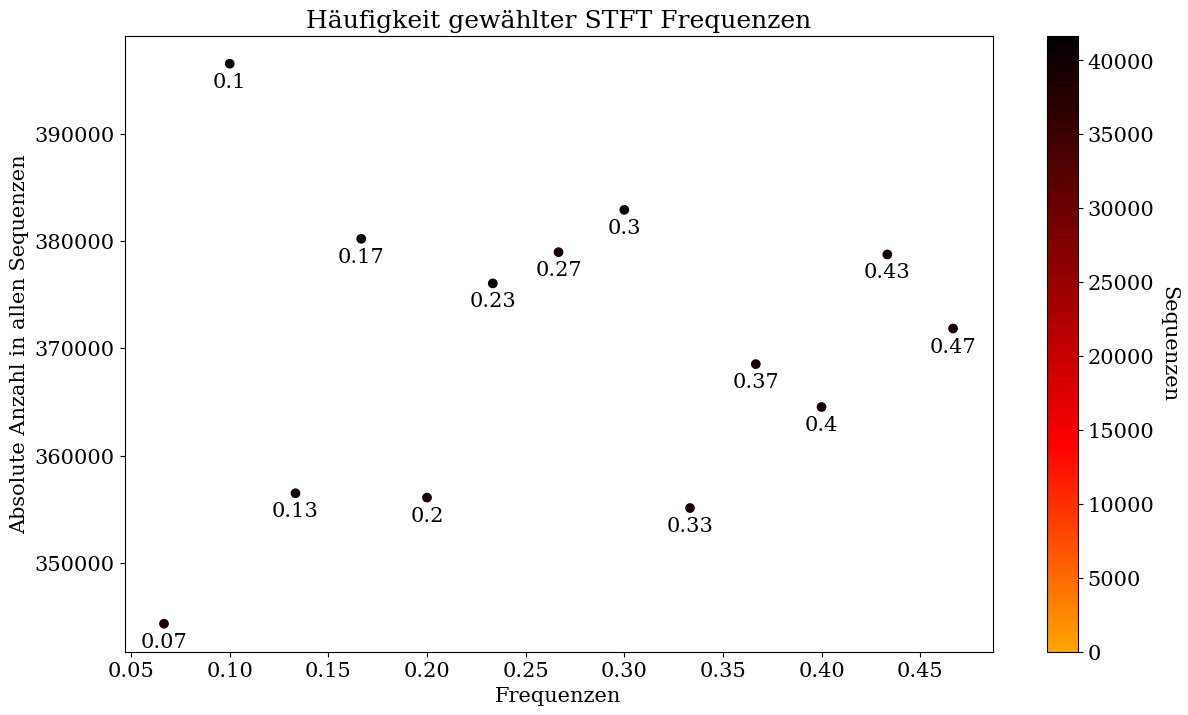
\includegraphics[width=\textwidth]{frequencies_normal.png}
                \caption{Normal}
                \label{fig:frequencies_normal}
            \end{subfigure}
            \caption[Häufigkeit gewählter Frequenzen über alle \aclp{TP} \Exp{exp:uniref90}]{Häufigkeit gewählter Frequenzen über alle \aclp{TP}: Die Häufigkeiten, wie oft eine Frequenz in einer Sequenz gewählt wird, werden über alle \ac{TP} summiert (y-Achse). Die Farbe der Punkte gibt an, in wie vielen Sequenzen die jeweilige Frequenz vorkam.}
            \label{fig:frequencies_uniref}
        \end{figure}

        Beim UniRef90 Sampling wurden die Amplituden-Grenzwerte für vier verschiedene Signifikanzniveaus ermittelt. \autoref{fig:frequencies_uniref} stellt den folglichen Einfluss auf die Frequenzselektion bezüglich Häufigkeit dar, exemplarisch für Hydrophobizität bei \ac{FG} 30 mit Überlappung von 15 und $n\_peaks = alle$.

        In \autoref{fig:frequencies_normal} ist die Auswahl vor dem Sampling dargestellt. Die Häufigkeiten der Frequenzen liegen im Mittel etwa bei 360000 und sind in allen Frequenzen vertreten, was bei circa 40000 Proteinen bedeutet, dass in einer Sequenz jede Frequenz etwa 9-mal vorkommt. Frequenz 0.1, also eine Periode von jeder 10. Aminosäure, scheint zudem besonders häufig gewählt zu werden. Bis auf \autoref{fig:frequencies_0.001} scheint das auch für die Frequenzselektion zu gelten, die auf dem Sampling basiert.

        Die Häufigkeiten werden mit schrumpfendem $\alpha$ deutlich kleiner. So kommt eine Frequenz mit 5\% Grenze nur etwa in jeder zweiten Sequenz vor, bei 0.1\% in jeder 20., und bei noch strengeren Grenzen seltener als in jeder 200. Sequenz.

        \begin{figure}[H]
            \centering
            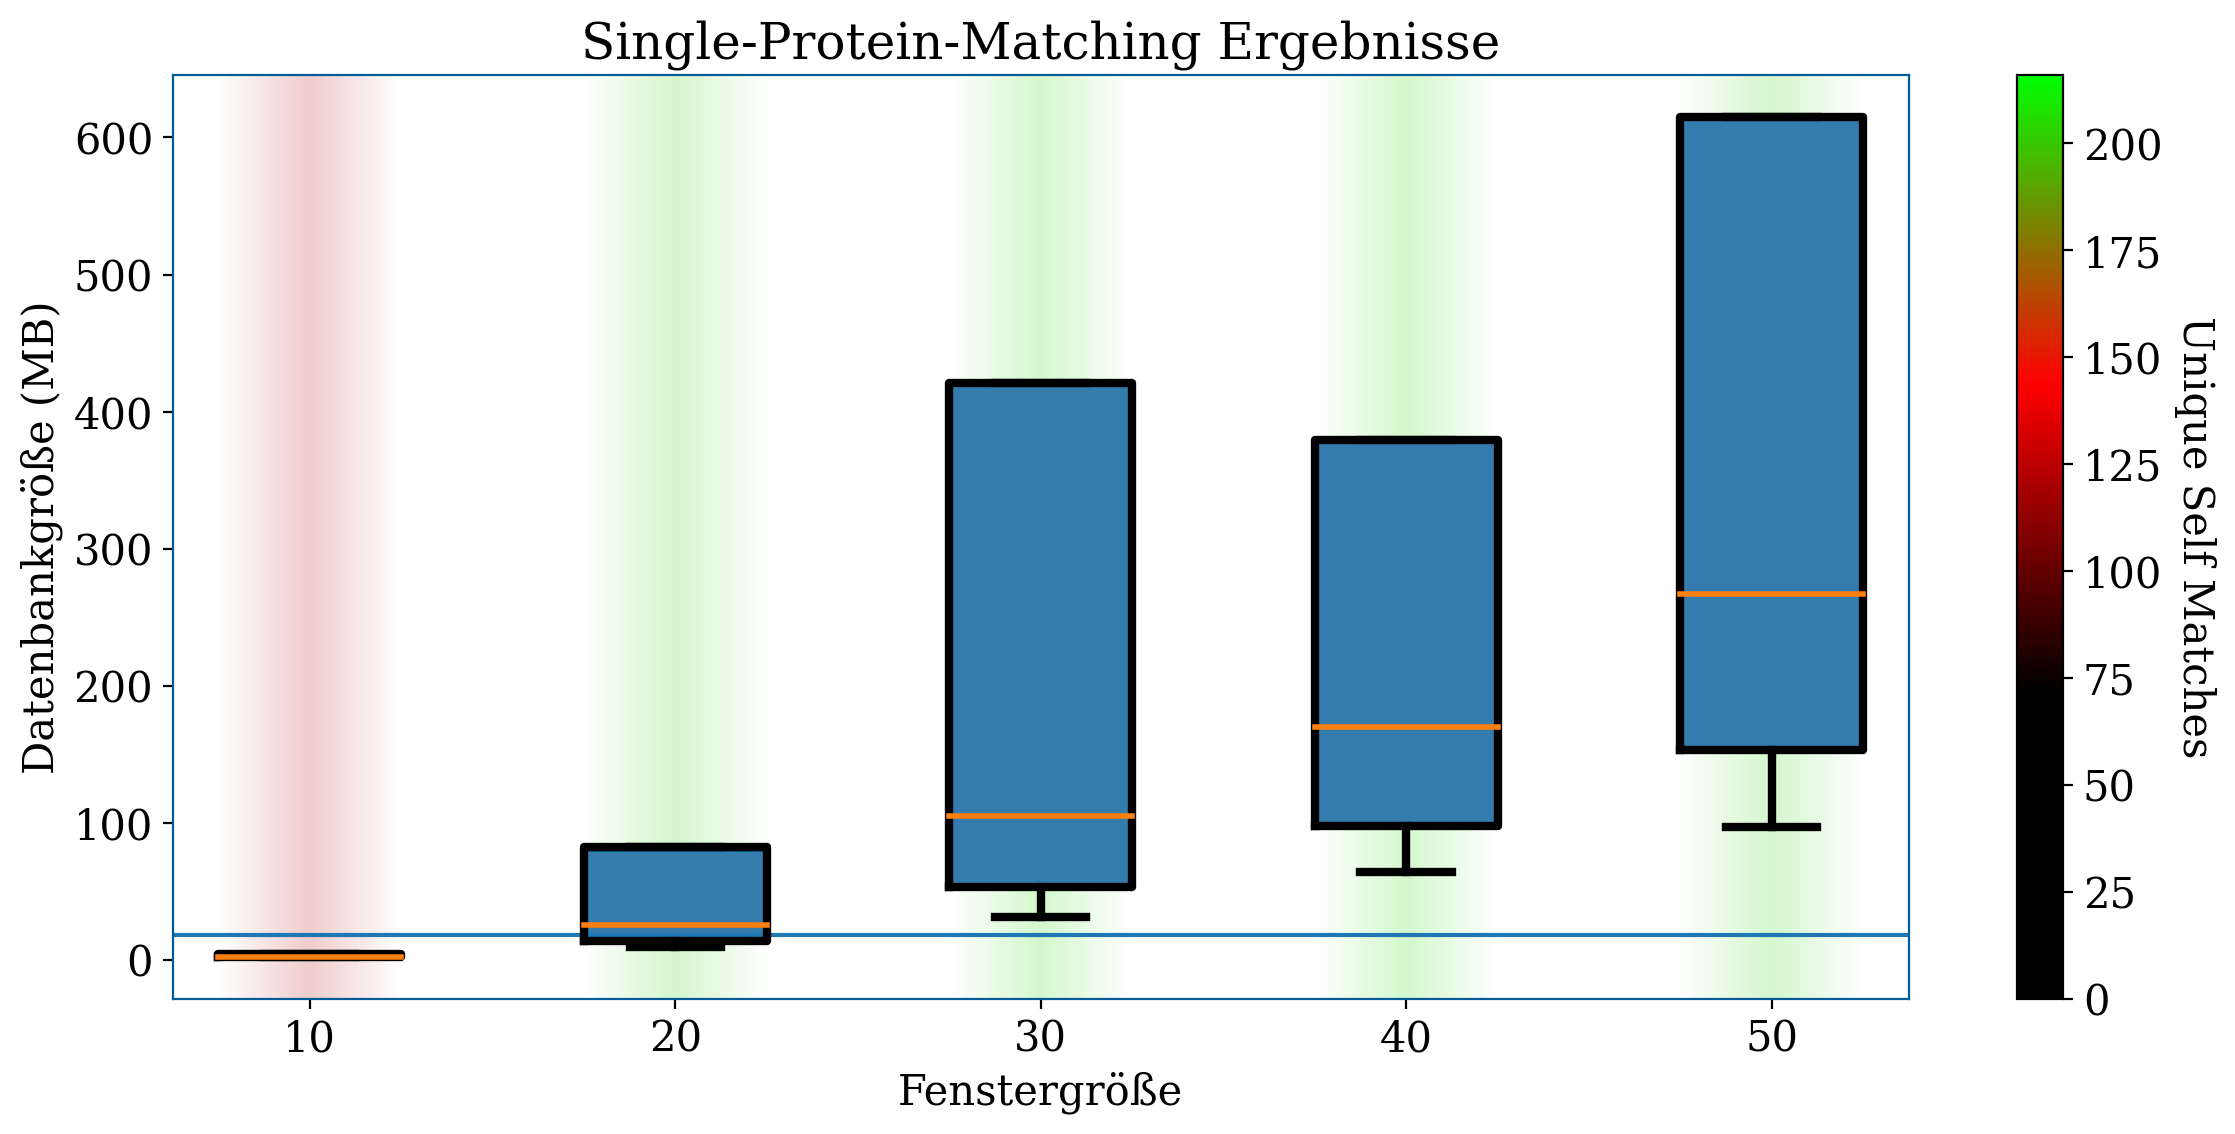
\includegraphics[width=\textwidth]{plot_uniref90.sp.png}
            \caption[Single-Protein-Matching \Exp{exp:uniref90}]{Matching-Ergebnisse für $\alpha=5\%$. Die Boxen bilden die Datenbankgrößen für die verschiedenen Parameter aus \autoref{tab:parameter} ab. Die blaue Füllung repräsentiert die Schärfe (\autoref{equ:f_score} \autopageref{equ:f_score}), sofern sie einen positiven Wert hat. Die farbige Fläche über und unter den Boxen stellt die Anzahl dar, wie viele der Suchproteine als Treffer mit alleinigem besten Score identifiziert wurden (hier ``Unique Self Matches''). Die blaue horizontale Linie kennzeichnet die Größe der Eingabedaten.}
            \label{fig:uniref90.sp}
        \end{figure}

        Ursprünglich war \autoref{exp:uniref90} so konzipiert, dass nur das ein 5\%-alpha ermittelt wird. Da die Datenbanken aber weiterhin zu groß sind, wie in \autoref{fig:uniref90.sp}, \autoref{sub:filter_results} und \autoref{sub:target_results} zu sehen, wurde es um die strengeren Signifikanzniveaus erweitert. Die Identifizierung ist ab \ac{FG} 20 sehr gut und hat eine nahezu 100\%-ige Schärfe. \ac{FG} 10 ist zwar unter der Eingabegröße, scheitert aber bei der Identifikation und wurde daher nicht für alle Experimente betrachtet. 
    
    % subsection uniref90_sampling (end)
    \subsection{Filter Hashes} % (fold)
        \label{sub:filter_results}
        Aufgrund eines Eingabefehlers wurde der Parameter $Quantil=0.8$ ausgelassen.

        \begin{figure}[H]
            \centering
            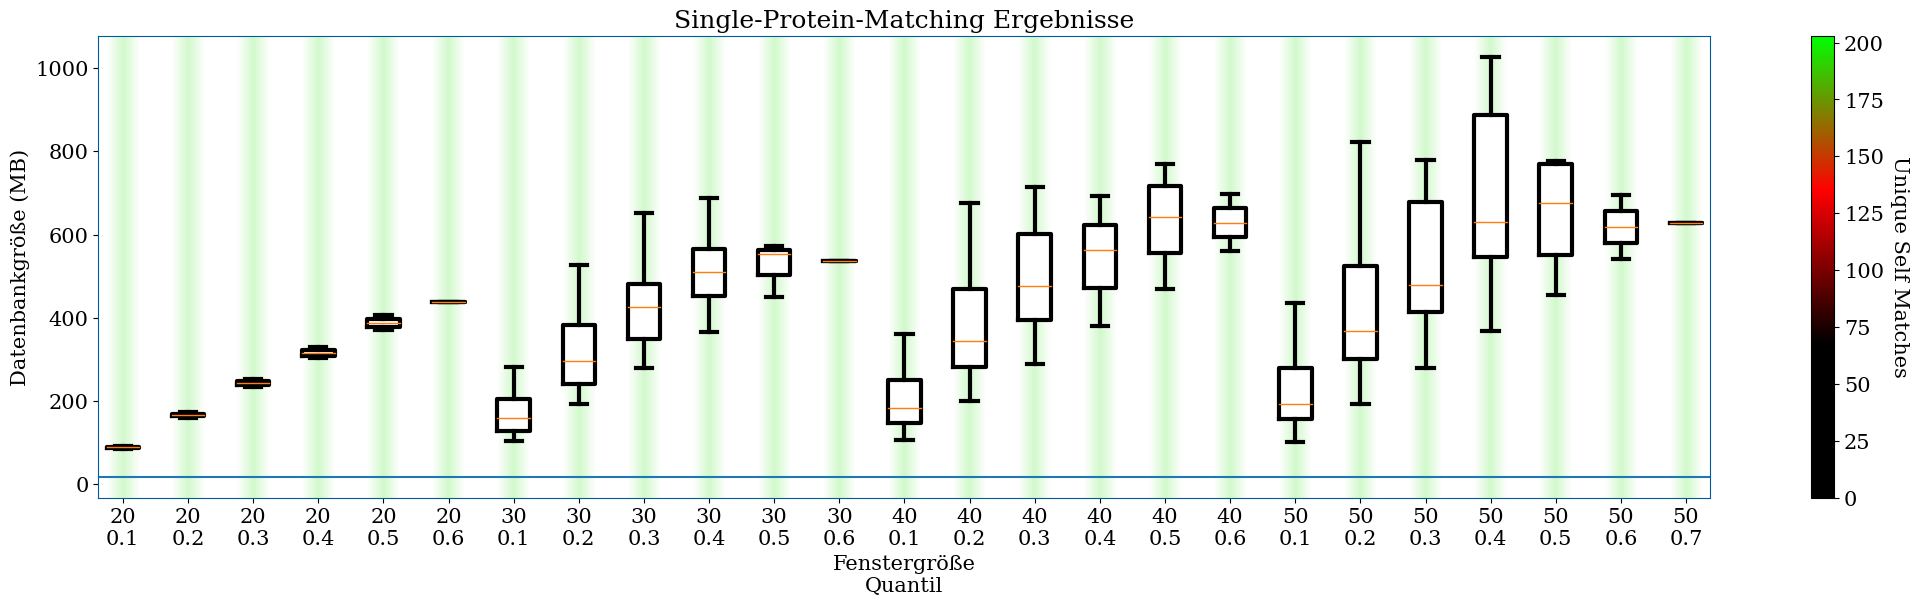
\includegraphics[width=\textwidth]{plot_filter_hashes.sp.png}
            \caption[Single-Protein-Matching \Exp{exp:filter_hashes}]{Die Boxen bilden die Datenbankgrößen für die verschiedenen Parameter aus \autoref{tab:parameter} ab. Die blaue Füllung repräsentiert die Schärfe (\autoref{equ:f_score} \autopageref{equ:f_score}), sofern sie einen positiven Wert hat. Die farbige Fläche über und unter den Boxen stellt die Anzahl dar, wie viele der Suchproteine als Treffer mit alleinigem besten Score identifiziert wurden (hier ``Unique Self Matches''). Die blaue horizontale Linie kennzeichnet die Größe der Eingabedaten.}
            \label{fig:filter_hashes.sp}
        \end{figure}

        Aufgrund zu langer Laufzeit wurde das Single-Protein-Matching vorzeitig abbgebrochen, sodass die Daten der pro \ac{FG} jeweils letzten Quantile nicht vollständig sind. \autoref{fig:filter_hashes.sp} zeigt für die Suchproteine für alle getesteten Parameter eine hohe Identifikationsrate mit hoher Schärfe. Mit sinkendem Quantil schrumpft auch die Datenbankgröße scheinbar linear. Dennoch ist keine davon unter dem Limit der Eingabe.

        \begin{figure}[H]
            \centering
            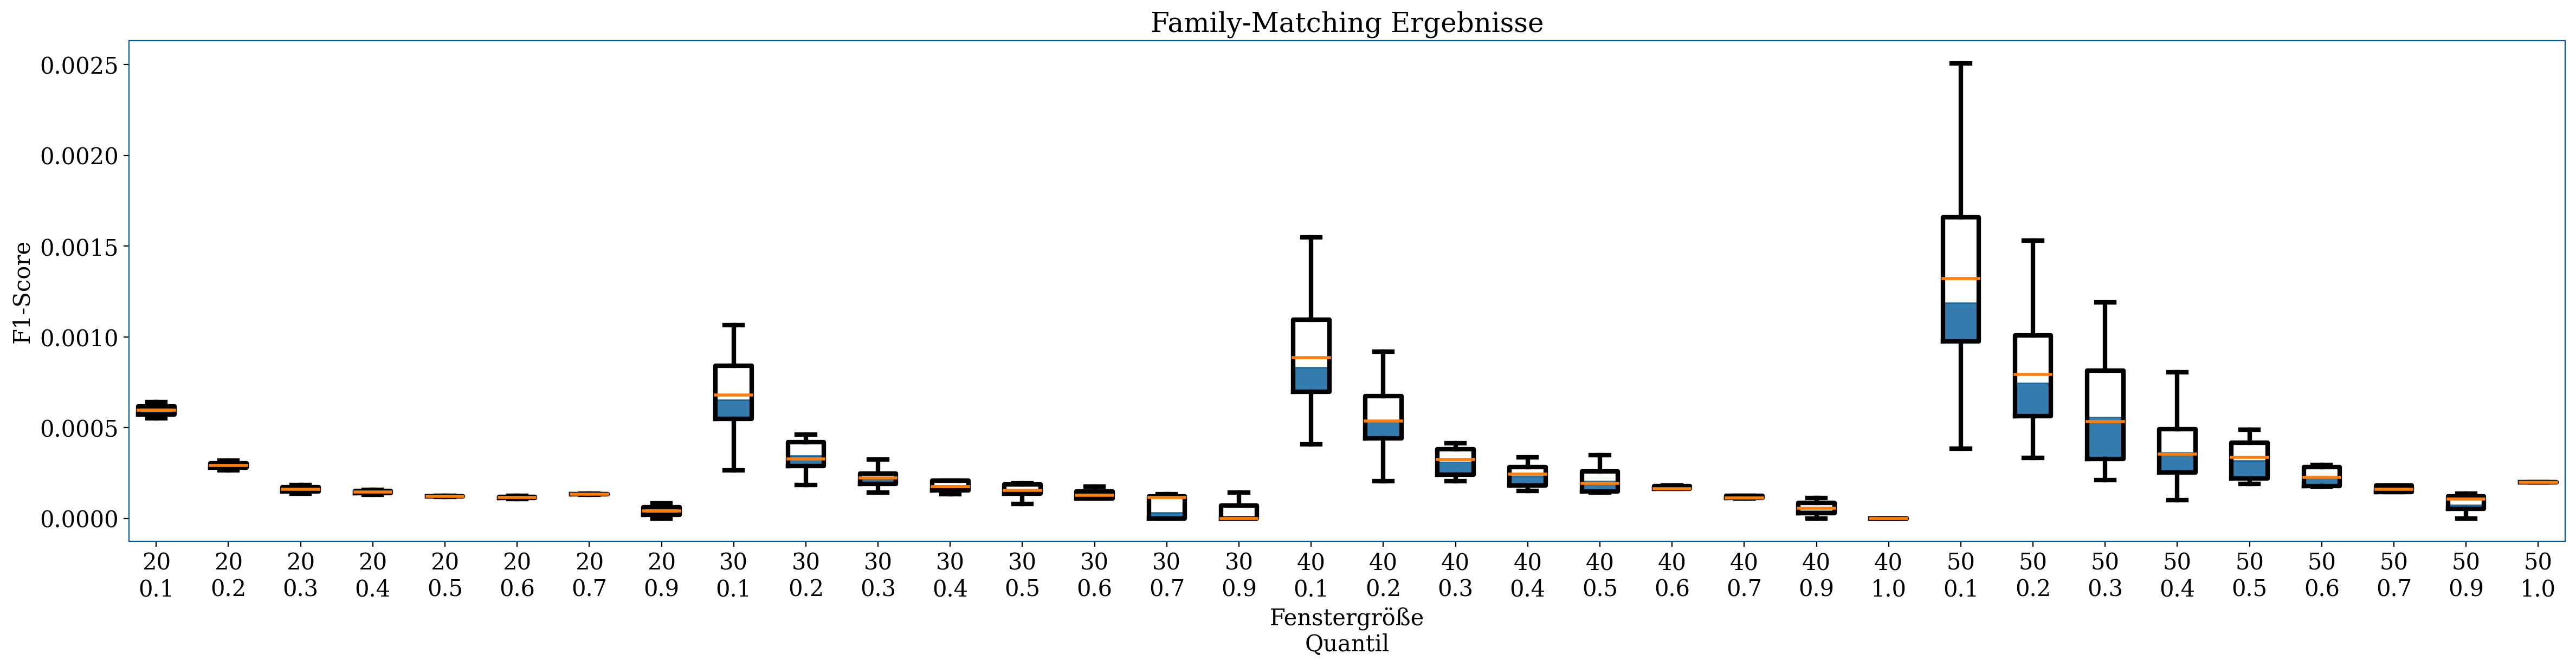
\includegraphics[width=\textwidth]{plot_filter_hashes.fam.png}
            \caption[Family-Matching \Exp{exp:filter_hashes}]{Die Boxen bilden die F-Scores für die verschiedenen Parameter aus \autoref{tab:parameter} ab. Die blaue Füllung repräsentiert die Schärfe (\autoref{equ:f_score} \autopageref{equ:f_score}), sofern sie einen positiven Wert hat.}
            \label{fig:filter_hashes.fam}
        \end{figure}

        Der Family-Matching-Ansatz in \autoref{fig:filter_hashes.fam} hat eine geringe Schärfe von unter 0.5, wobei sich für die getesteten Parameter zeigt, dass kleinere Quantile einen höheren F-Score haben, der aber deutlich unter 1 liegt.

    \subsection{Target-Zone} % (fold)
        \label{sub:target_results}
        \begin{figure}[H]
            \centering
            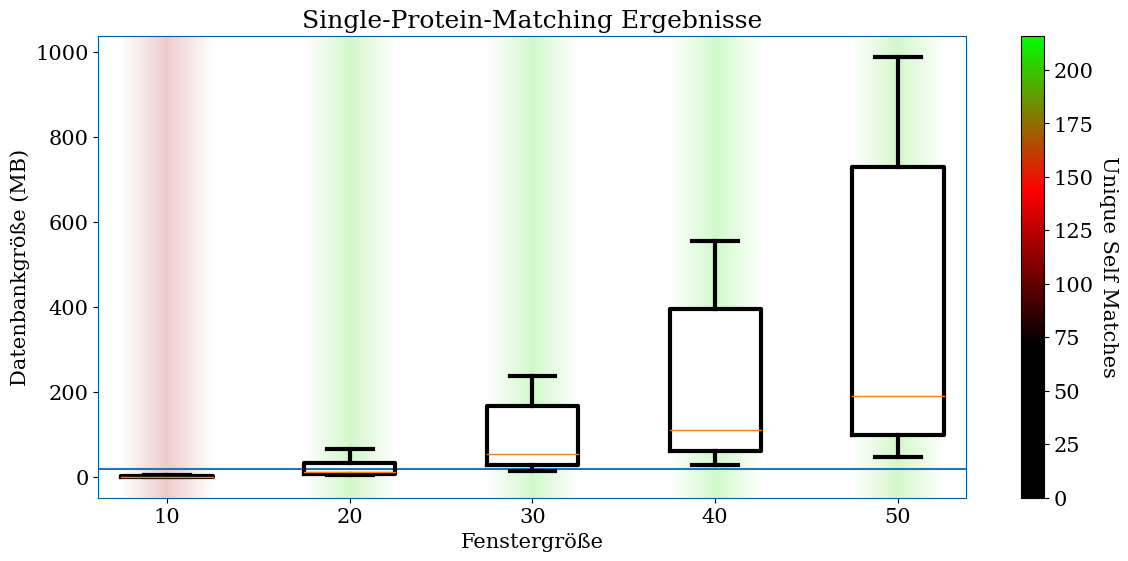
\includegraphics[width=\textwidth]{plot_target_zone.sp.png}
            \caption[Single-Protein-Matching \Exp{exp:target_zone}]{Die Boxen bilden die Datenbankgrößen für die verschiedenen Parameter aus \autoref{tab:parameter} ab. Die blaue Füllung repräsentiert die Schärfe (\autoref{equ:f_score} \autopageref{equ:f_score}), sofern sie einen positiven Wert hat. Die farbige Fläche über und unter den Boxen stellt die Anzahl dar, wie viele der Suchproteine als Treffer mit alleinigem besten Score identifiziert wurden (hier ``Unique Self Matches''). Die blaue horizontale Linie kennzeichnet die Größe der Eingabedaten.}
            \label{fig:target_zone.sp}
        \end{figure}

        Für das Testen verschiedener \aclp{TZ} ist in \autoref{fig:target_zone.sp} eine Tendenz zu exponentiellem Wachstum der Datenbankgröße bei ansteigender \ac{TZ} erkennbar. Wie beim Sampling in \autoref{fig:uniref90.sp} scheitert die Identifikation bei \ac{FG} 10, im Gegensatz zu den anderen Größen, welche auch eine hohe Schärfe haben.

    \subsection{Selection-Method} % (fold)
        \label{sub:selection_results}
        Da das \autoref{exp:target_zone} in \autoref{sub:target_results} aufgrund zu hoher Laufzeit vorzeitig abgebrochen wurde, wurde in dem hiesigen Experiment die Datenbankerstellung bei zu hoher Größe abgebrochen. Lediglich der Selektionsansatz, der die Maxima der absoluten Grenzwertabweichungen auswählt, hat zur Fertigstellung geführt, sodass das Matching nur für diese Datenbanken erfolgen konnte.

        Die vorigen Ergebnisse haben veranlasst, wie in \autoref{sub:uniref90_results} erwähnt, das Signifikanzniveau von 5\% zu verringern, sodass zusätzlich die Grenzwerte für $\alpha \in \{0.1, 0.01, 0.001\}$ ermittelt wurden. Um die Laufzeit dieses Experiments durch zu viele Parameterwerte nicht unnötig zu erhöhen, wurden vor der Durchführung die pro \ac{TP} selektierten Frequenzen gezählt und die mittlere Anzahl Frequenzen pro Fenster ermittelt, um die zu testenden $\alpha$-Werte zu begrenzen.

        \begin{figure}
             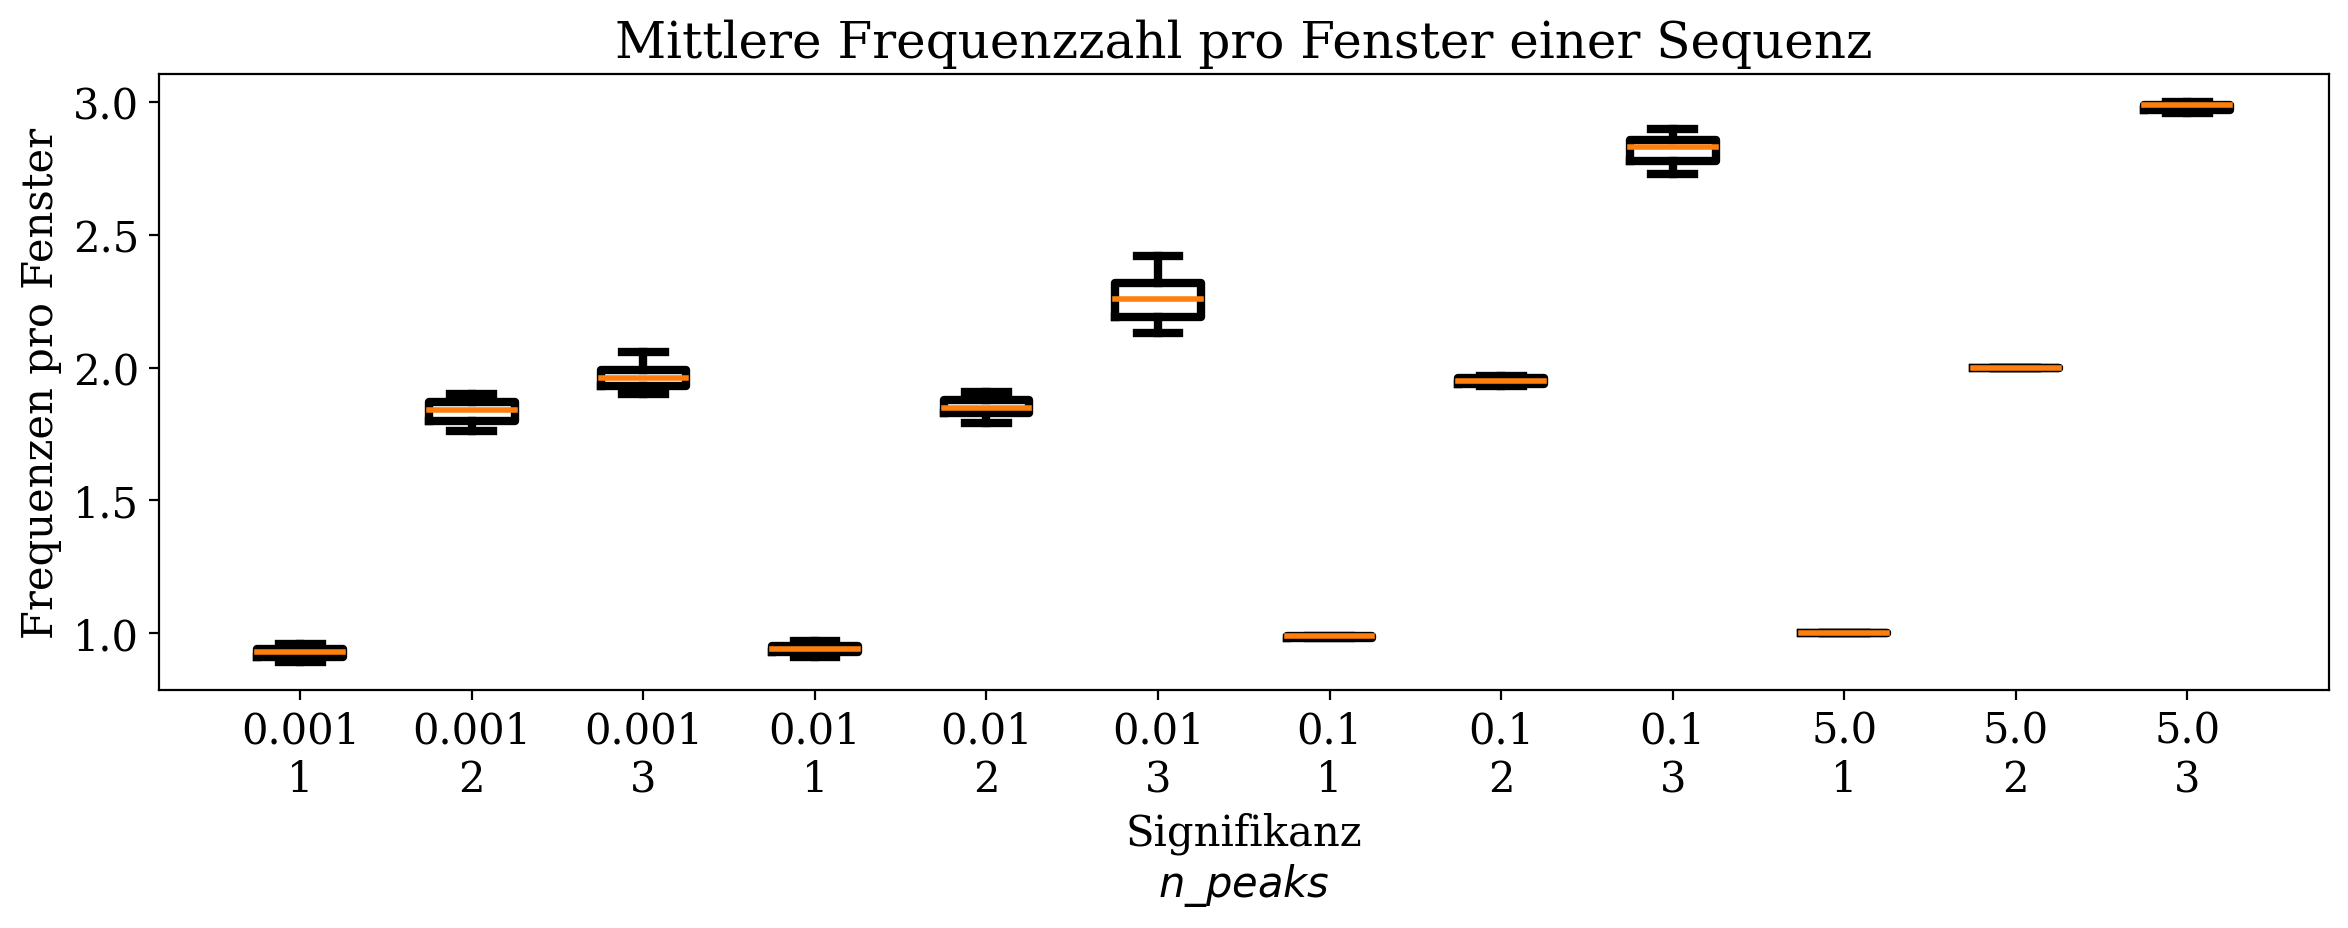
\includegraphics[width=\textwidth]{plot_mean_frequencies.png}
             \caption{Mittlere Frequenzzahl pro Fenster einer Sequenz}
             \label{fig:mean_frequencies}
        \end{figure} 

        In \autoref{fig:mean_frequencies} wird deutlich, dass die Verringerung der Signifikanz die Anzahl der gewählten Frequenzen reduziert. Für $\alpha=5\%$ sind es deutlich zu viele Frequenzen, da die Anzahl aufgrund der geringen Streuung offenbar lediglich durch $n\_peaks$ limitiert wird. Wenn eine Datenbank nicht größer als die Eingabe sein soll, dürfen die Daten einer Sequenz nicht den Speicherbedarf der Textrepräsentation ihrer Aminosäuren überschreiten. Diese Zeichen sind Teil des \ac{ASCII} und benötigen daher nur 1 Byte Speicher, was bedeutet, dass bei einer Sequenz der \ac{TP} mit einer medialen Länge von etwa 300 Aminosäuren nur ebensoviele Bytes verwendet werden dürften. Hierzu eine Rechnung unter der Annahme, es gäbe nur eine Frequenz pro Fenster:
        \begin{equation}
            \begin{split}
                target\_zone &= 8\\
                \emph{fenster\_größe} &= 30\\
                \emph{überlappung} &= 15\\
                \emph{sequenz\_länge} &= 300\\
                anzahl\_fenster &= \frac{\emph{sequenz\_länge}}{\emph{fenster\_größe} - \emph{überlappung}} = 20\\
                \emph{hash\_größe} &= 32 Bit = 4 Byte\\
                speicher\_pro\_kf &= target\_zone * anzahl\_fenster * \emph{hash\_größe} = 640\ Byte\\
                anzahl\_kf = 10\\
                datenbank\_speicher &= target\_zone * anzahl\_fenster * \emph{hash\_größe} * 10 = 6400\ Byte
            \end{split}
        \end{equation}

        Selbst bei einer Frequenz pro Fenster wäre die Datenbank nach dieser Abschätzung doppelt so groß wie die Eingabe. Von daher sollte $\alpha$ die Frequenzwahl möglichst in Richtung einer Anzahl von 1 bringen, weshalb $\alpha=0.1$ nicht verwendet wird, da die Streuung hier auf meistens 2 Frequenzen pro Fenster schließen lässt. Das Matching wird von daher für die beiden kleinsten $\alpha$-Werte durchgeführt.

        \begin{figure}[H]
            \centering
            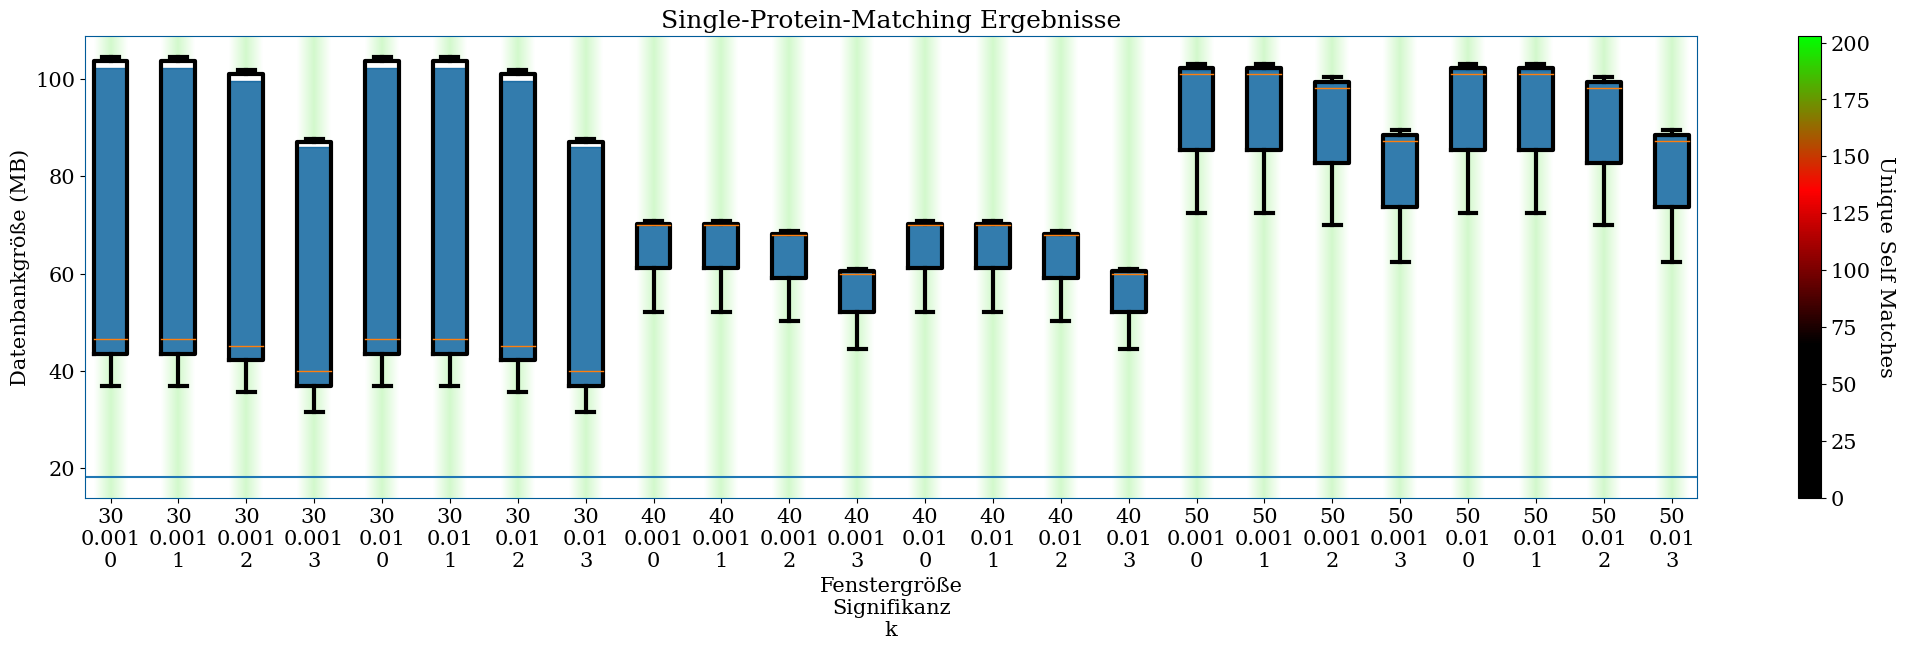
\includegraphics[width=\textwidth]{plot_selection_method.sp.png}
            \caption[Single-Protein-Matching \Exp{exp:selection_method}]{Die Boxen bilden die Datenbankgrößen für die verschiedenen Parameter aus \autoref{tab:parameter} ab. Die blaue Füllung repräsentiert die Schärfe (\autoref{equ:f_score} \autopageref{equ:f_score}), sofern sie einen positiven Wert hat. Die farbige Fläche über und unter den Boxen stellt die Anzahl dar, wie viele der Suchproteine als Treffer mit alleinigem besten Score identifiziert wurden (hier ``Unique Self Matches''). Die blaue horizontale Linie kennzeichnet die Größe der Eingabedaten.}
            \label{fig:selection_method.sp}
        \end{figure}

        In \autoref{fig:selection_method.sp} zeigt sich für das Single-Protein-Matching, dass die Identifikation bei den getesteten Parametern mit hoher Schärfe erfolgreich funktionierte. Beim Wechsel von $k=2$ zu $k=3$ ist zudem ein kleiner Sprung nach unten zu erkennen.

        \begin{figure}[H]
            \centering
            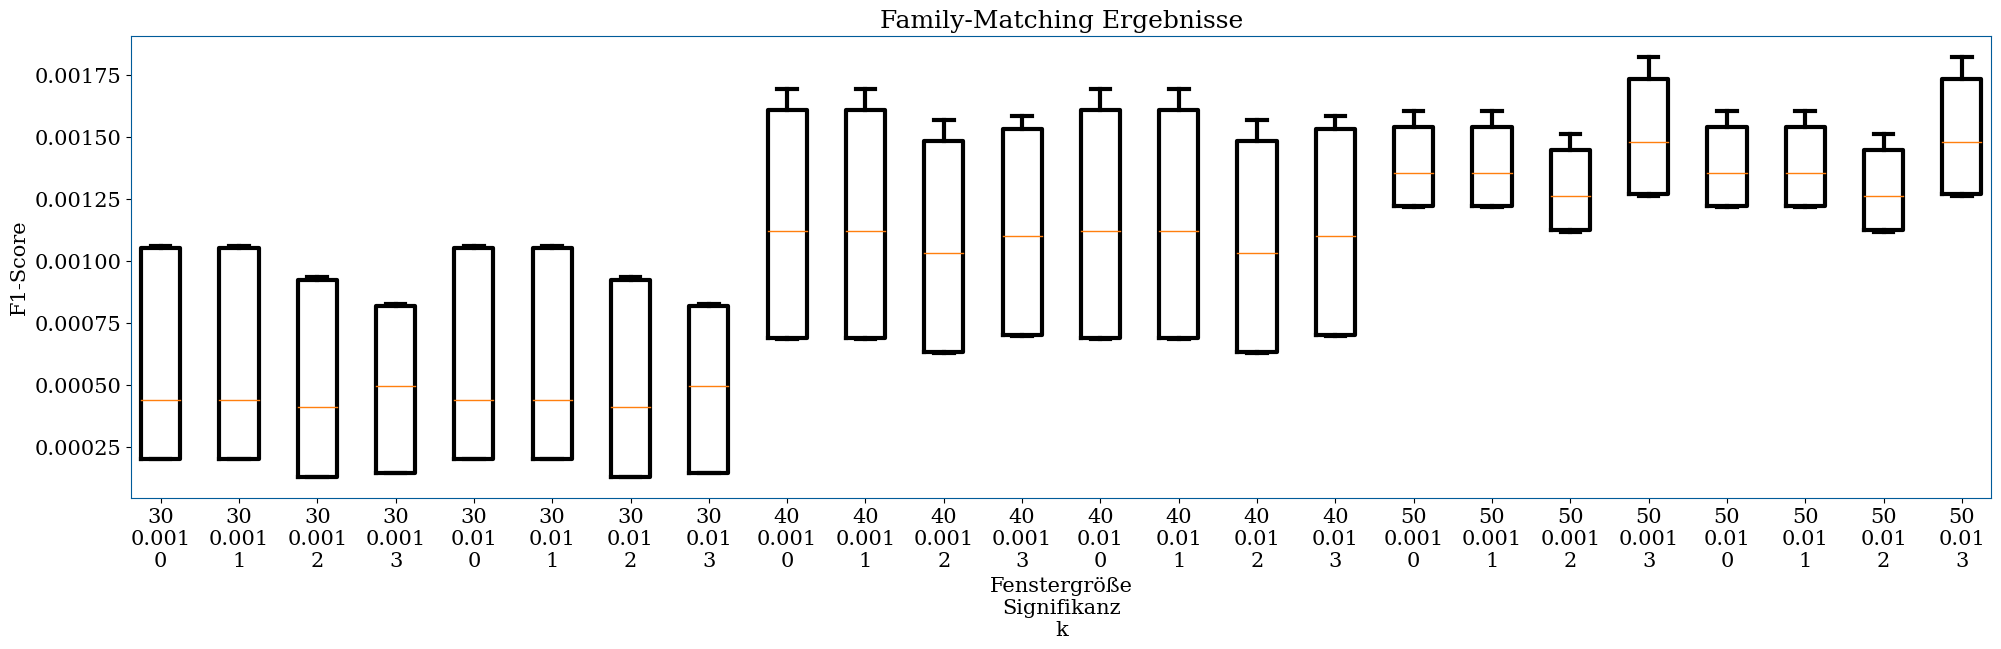
\includegraphics[width=\textwidth]{plot_selection_method.fam.png}
            \caption[Family-Matching \Exp{exp:selection_method}]{Die Boxen bilden die F-Scores für die verschiedenen Parameter aus \autoref{tab:parameter} ab. Die blaue Füllung repräsentiert die Schärfe (\autoref{equ:f_score} \autopageref{equ:f_score}), sofern sie einen positiven Wert hat.}
            \label{fig:selection_method.fam}
        \end{figure}

        Beim Family-Matching scheinen die höheren \acp{FG} ab 40 besser abzuschneiden. Für $k=2$ sinkt der F-Score ein wenig. Die Schärfe liegt wie bei \autoref{fig:filter_hashes.fam} überall unter $0.5$.
% section ergebnisse (end)
